\documentclass[lang=cn,10pt]{elegantbook}

\title{计算机图形学基础}
\subtitle{第五版 \  中文译本}
\author{Steve Marschner \& Peter Shirley}
\institute{Cornell University \& NVIDIA}
\date{February 2021}
\version{Fifth edition}
\bioinfo{译者}{buding}

\extrainfo{Stay hungry. Stay foolish. —— Steve Jobs}

\setcounter{tocdepth}{1}

\logo{CRC.png}
\cover{cover.png}

% 本文档命令
\usepackage{array}
\setCJKmainfont[Path=fonts/]{LXGWWenKai-Regular.ttf}
\definecolor{lightgreen}{RGB}{99,140,94}
\newcommand{\ccr}[1]{\makecell{{\color{#1}\rule{1cm}{1cm}}}}

% 修改标题页的橙色带
\definecolor{customcolor}{RGB}{171,35,74}
\colorlet{coverlinecolor}{customcolor}

\begin{document}

\maketitle

\frontmatter

\chapter{前言}

本版的《计算机图形学基础》包括对阴影着色、光线反射和路径追踪等材料的大量重写,以及对全书谬误的许多订正。本书对基于物理的材料和基于物理的渲染等技术进行了更好的介绍,这些技术在实际应用中逐渐占据主导地位。现在这些材料得到了更好的整合,我们认为这本书很好地匹配了目前许多教师组织图形学课程的方式。  

本书的组织结构与第四版基本相似。在多年来对本书进行修订的过程中,我们努力保留了早期版本中非正式的、直观的表述风格,同时也提高了本书的一致性、准确性和完整性。我们希望读者能够发现,本书是一个吸引人的平台,适合于各种计算机图形学课程。

\section*{关于封面}

封面图片来自 J.W.Baker 的《水中之虎》(画布上的拉丝和喷枪亚克力,16英寸x20英寸),www.jwbart.com。  

老虎的主题是指 Alain Fournier(1943-2000)1998年在康奈尔大学的一次研讨会上的精彩演讲。他的演讲是对老虎动作进行的令人回味的口头描述。他总结了自己的观点:  

尽管在过去的35年里,计算机图形学的建模和渲染已经有了巨大的进展,但我们仍然无法自动模拟在河中游泳的老虎所有精彩细节。我所说的自动是指不需要艺术家或专家进行仔细的手动调整的方式。    

坏消息是,我们还有很长的路没走。  

好消息是,我们还有很长的路要走。

\section*{线上资源}

本书的网址是 http://www.cs.cornell.edu/\~{}srm/fcg5/ 。我们将继续维护本书的勘误表和课程链接,以及与本书风格相符的教学材料。本书中的大多数图片都是 Adobe Illustrator 格式的,我们很乐意根据需要将特定图片转换为可移植格式。请随时通过 srm@cs.cornell.edu 或 ptrshrl@gmail.com 与我们联系。  

\chapter{致谢}

以下人士提供了对于本书各版本的有用信息、评论或者反馈:Ahmet O˘guz Aky¨uz, Josh Andersen, Beatriz Trinch˜ao Andrade Zeferino Andrade, Bagossy Attila, Kavita Bala, Mick Beaver, Robert Belleman, Adam Berger, Adeel Bhutta, Solomon Boulos, Stephen Chenney, Michael Coblenz, Greg Coombe, Frederic Cremer, Brian Curtin, Dave Edwards, Jonathon Evans, Karen Feinauer, Claude Fuhrer, Yotam Gingold, Amy Gooch, Eungyoung Han, Chuck Hansen, Andy Hanson, Razen Al Harbi, Dave Hart, John Hart, Yong Huang, John “Spike” Hughes, Helen Hu, Vicki Interrante, Wenzel Jakob, Doug James, Henrik Wann Jensen, Shi Jin, Mark Johnson, Ray Jones, Revant Kapoor, Kristin Kerr, Erum Arif Khan, Mark Kilgard, Fangjun Kuang, Dylan Lacewell, Mathias Lang, Philippe Laval, Joshua Levine, Marc Levoy, Howard Lo, Joann Luu, Mauricio Maurer, Andrew Medlin, Ron Metoyer, Keith Morley, Eric Mortensen, Koji Nakamaru, Micah Neilson, Blake Nelson, Michael Nikelsky, James O’Brien, Hongshu Pan , Steve Parker, Sumanta Pattanaik, Matt Pharr, Ken Phillis Jr, Nicol`o Pinciroli, Peter Poulos, Shaun Ramsey, Rich Riesenfeld, Nate Robins, Nan Schaller, Chris Schryvers, Tom Sederberg, Richard Sharp, Sarah Shirley, Peter-Pike Sloan, Hannah Story, Tony Tahbaz, JanPhillip Tiesel, Bruce Walter, Alex Williams, Amy Williams, Chris Wyman, Kate Zebrose, and Angela Zhang。  

Ching-Kuang Shene 和 David Solomon 允许我们借用他们的例子。 Henrik Wann Jensen、Eric Levin、Matt Pharr 和 Jason Waltman 慷慨地提供了图片。 Brandon Mansfield 帮助改进了关于光线追踪的分层包围体的探讨。 Philip Greenspun (philip.greenspun.com) 热心地允许我们使用他的照片。 John “Spike” Hughes 帮助改进了对抽样理论的探讨。 Wenzel Jakob 的 Mitsuba 渲染器在创建许多图形方面非常宝贵。我们非常感谢 J.W. Baker 帮助创作了 Pete 设想的封面。他除了是一位才华横溢的艺术家之外,也是一位非常愉快的工作伙伴。  

本书的章节注释中引用了许对编写本书有帮助的著作。然而,有几本影响了本书内容和表现形式的关键文献值得在此特别表彰。其中包括两本经典的计算机图形学教材,我们都是从这两本教材中学习的基础知识——《计算机图形学:原理与实践》(Foley、Van Dam、Feiner 和 Hughes,1990 年)和《计算机图形学》(Hearn 和 Baker,1986 年)。其他文本包括 Alan Watt 的两本有影响力的书籍 (Watt, 1993, 1991), Hill的《使用OpenGL的计算机图形》(Francis S. Hill, 2000), Angel的《交互式计算机图形学:使用 OpenGL 的自上而下方法》(Angel, 2002), Hugues Hoppe 的华盛顿大学论文 (Hoppe, 1994) 和 Rogers 的两篇优秀的图形学文章 (D. F. Rogers, 1985, 1989)。  

我们要特别感谢 Alice 和 Klaus Peters 鼓励 Pete 撰写本书的第一版,感谢他们在帮助完成本书方面的伟大才能。他们对作者的耐心以及竭尽所能奉献于使本书成为最好的书籍对本书的出版起了重要的作用。如果没有他们的非凡努力,这本书肯定不会存在。 

\rightline{Steve Marschner,伊萨卡,纽约}

\rightline{Peter Shirley,盐湖城,犹他州}

\rightline{2021年2月}

\chapter{作者}

Steve Marschner是康奈尔大学的计算机科学教授。他于1993年在布朗大学获得理学学士学位,1998年在康奈尔大学获得博士学位。在2002年加入康奈尔大学之前,他在微软研究院和斯坦福大学担任研究职务。他是2015年SIGGRAPH计算机图形学成就奖的获得者和2003年技术学院奖的共同获得者。

Peter Shirley是英伟达公司的杰出研究科学家。他曾在印第安纳大学、康奈尔大学和犹他大学担任学术职务。他于1985年获得里德学院的物理学学士学位,1991年获得伊利诺伊大学的计算机科学博士学位。

\tableofcontents

\mainmatter

\chapter{图形学介绍}

计算机图形学这个术语描述了任何使用计算机来创建和操作图像的情况。本书介绍了可用于创建各种图像的算法和数学工具——逼真的视觉效果、丰富的技术插图或精美的计算机动画。图形可以是二维的,也可以是三维的;图像可以是完全合成的,也可以是通过处理照片产生的。本书是关于基本算法和数学的,特别是那些用于制作三维物体和场景的合成图像的算法。

实际上,做计算机图形不可避免地需要了解特定的硬件、文件格式,通常还需要一个或两个图形API(参见1.3节)。计算机图形学是一个快速发展的领域,因此这些知识的具体内容是在不断更新变化。因此,在本书中,我们尽力避免依赖任何特定的硬件或API。我们鼓励读者用他们的软件和硬件环境的相关文档来补充此文本。幸运的是,计算机图形文化有足够的标准术语和概念,本书的讨论应能很好地反映到大多数环境。


\remark{ API:应用程序编程接口}  

本章定义了一些基本术语,并提供了一些历史背景,以及与计算机图形相关的信息来源。

\section{图形学领域}

对任何领域强加分类都是危险的,但大多数图形从业者会对计算机图形的以下主要领域达成一致:

\begin{itemize}
\item 建模涉及的是形状和外观属性的数学规范化,这种方式可以存储在计算机上。例如,可以将咖啡杯描述为一组有序的三维点,以及一些连接这些点的插值规则和一个描述光线如何与杯子作用的反射模型。
\item 渲染是一个从艺术中继承下来的术语,涉及到从三维计算机模型创建阴影图像。
\item 动画是一种通过图像序列创造运动幻觉的技术。动画使用建模和渲染,但增加了随着时间移动的关键问题,这在基本的建模和渲染中通常无法处理。
\end{itemize}

还有许多其他涉及计算机图形的领域,关于它们是否属于图形学的核心领域,仁者见仁,智者见智。这些内容在本书都至少有所提及。此类相关领域包括以下内容:
\begin{itemize}
\item 用户接口涉及输入设备,例如鼠标和平板电脑、应用程序、图像对用户的反馈以及其他感官反馈的接口。从历史上看,该领域与图形有关,主要是因为计算机图形的研究人员最早接触到了现在无处不在的输入和输出设备。
\item 虚拟现实试图让用户沉浸在一个三维虚拟世界中。这通常要求至少有立体图形和对头部运动的反应。对于真正的虚拟现实,还应该提供声音和力量的反馈。因为这一领域需要先进的三维图形和先进的显示技术,所以它通常与图形学密切相关。
\item 可视化试图通过视觉显示让用户深入了解复杂的信息。通常,在一个可视化问题中,有一些图形问题需要解决。
\item 图像处理涉及对二维图像的操作,在图形和视觉领域均有应用。
\item 三维扫描使用测距技术来创建被评估的三维模型。这类模型对于创造丰富的视觉图像很有帮助,而处理这种模型往往需要图形算法。
\item 计算摄影是使用计算机图形、计算机视觉和图像处理方法,以实现拍摄物体、场景和环境的新方法。
\end{itemize}

\section{主要应用}

几乎任何工作都可以在一定程度上使用计算机图形,但计算机图形技术的主要消费者包括以下行业:

\begin{itemize}
\item 视频游戏越来越多地使用复杂的三维模型和渲染算法。
\item 卡通片通常是直接由三维模型渲染。许多传统的二维卡通片使用由三维模型的背景渲染,这使得连续移动的视角不需要大量花费艺术家时间。
\item 视觉效果几乎使用了所有类型的计算机图形技术。几乎每部现代电影都使用数字合成技术,将背景与单独拍摄的前景叠加。许多电影还使用三维建模和动画来创造合成环境、物体甚至人物,而大多数观众都不会怀疑这不是真的。
\item 动画片使用了许多与视觉效果相同的技术,但不一定要追求图像的真实性。
\item CAD/CAM是指计算机辅助设计和计算机辅助制造。这些领域利用计算机技术在计算机上设计零件和产品,然后利用这些虚拟设计来指导制造过程。例如,许多机械零件是在三维计算机建模软件包中设计的,然后在计算机控制的铣削设备上自动生产。
\item 仿真可以被认为是精确的视频游戏。例如,飞行模拟器使用复杂的三维图形来模拟驾驶飞机的体验。这样的模拟对于安全关键领域的初始培训,例如驾驶汽车,以及对于有经验的用户的场景培训都是非常有用的,如在实际操作中成本太高或太危险的特定灭火情况。
\item 医学影像为扫描的病人数据创建有意义的图像。例如,计算机断层扫描(CT)数据集是由密度值的大型三维矩阵组成。计算机图形被用来创建阴影图像,帮助医生从这些数据中提取最突出的信息。
\item 信息可视化创造的数据图像不一定具有“自然”的视觉描述。例如,十只不同股票价格的时间趋势没有明显的视觉描述,但巧妙的图形技术可以帮助人类看到这些数据的模式。
\end{itemize}

\section{图形API}

使用图形库的一个关键部分是处理图形API。应用程序接口(API)是执行一系列相关操作的标准函数集合,而图形API是执行如将图像和三维表面绘制到屏幕上的窗口等基本操作的函数集合。

每个图形程序都需要能够使用两个相关的API:一个图形API用于视觉输出,一个用户界面API用于从用户那里获得输入。目前有两种主流的图形和用户界面API范式。第一种是集成的方法,以Java为例,其中图形和用户界面工具包是集成的、可移植的包,作为语言的一部分得到完全的标准化和支持。第二种是以Direct3D和OpenGL为代表的,其中绘图命令是与C++等语言相联系的软件库的一部分,而用户界面软件是一个独立的实体,可能因系统而异。在后一种方法中,编写可移植的代码是有问题的,尽管对于简单的程序,可能会使用可移植的库层来封装系统特定的用户界面代码。

无论你选择什么样的API,基本的图形调用将大致相同,而且本书的概念也适用。

\section{图形管道}

现在的每台台式电脑都有一个强大的三维图形管道。这是一个特殊的软件/硬件子系统,可以有效地绘制透视的三维图元。通常,这些系统针对处理具有共享顶点的三维三角形进行了优化。管道中的基本操作是将三维顶点位置映射到二维屏幕位置,并对三角形进行着色,以使它们看起来既逼真又以适当的从后到前(back-to-front)的顺序出现。

尽管按照有效的从后到前顺序绘制三角形曾经是计算机图形学中最重要的研究问题,但现在几乎都是用z-buffer来解决,它使用一个特殊的内存缓冲区,以蛮力的方式解决问题。

事实证明,图形管道中使用的几何操作几乎可以完全在四维坐标空间中完成,该空间由三个传统的几何坐标和第四个有助于透视的齐次坐标组成。这些四维坐标是用 $4 \times 4$ 矩阵和4矢量来操作的。因此,图形管道包含了许多有效处理和合成这些矩阵和矢量的机制。这种四维坐标系是计算机科学中最微妙和美丽的结构之一,无疑也是学习计算机图形学时需要跨越的最大智力障碍。每本图形学书籍的第一部分都有很大一部分是关于这些坐标的。

生成图像的速度在很大程度上取决于绘制三角形的数量。因为在许多应用中,交互性比视觉质量更重要,所以尽量减少用于表示模型的三角形数量是值得的。此外,如果从远处看模型,需要的三角形数量比从近处看模型时少。这表明,使用不同的细节级别(LOD)来表示一个模型是很有用的。

\section{数值问题}

许多图形程序实际上只是三维数字代码。数字问题在这类程序中往往是至关重要的。在 "过去",要以健壮和可移植的方式处理这些问题是非常困难的,因为机器对数字有不同的内部表示,更糟糕的是,处理异常的方式也不尽相同,互不兼容。幸运的是,几乎所有的现代计算机都符合IEEE浮点标准(IEEE标准协会,1985)。这允许程序员对处理某些数字条件做出许多方便的假设。

\remark{ IEEE浮点运算有两种零的表示方法,一种被视为正数,另一种被视为负数。虽然-0和+0之间的区别只是偶尔会出现,但是在这种情况下还是值得记住的。}

尽管IEEE浮点具有很多在编码数值算法时很有价值的特性,但对于图形中遇到的大多数情况只有少数几个特性是至关重要的。首先,也是最重要的是要了解IEEE浮点运算中实数的三个"特殊 "值。

1. 无穷大($\infty$)。这是一个比其他所有有效数字都大的有效数字。

2. 负无穷大($-\infty$)。这是一个比其他所有有效数字都小的有效数字。

3. 不是一个数字($\mathrm{NaN}$)。这是一个无效的数字,是由一个具有不确定后果的操作产生的,如0除以0。

IEEE浮点数的设计者做出了一些对程序员来说非常方便的决定。其中许多与上述三个处理异常的特殊值有关,比如除以零。在这些情况下,异常会被记录下来,但在很多情况下,程序员可以忽略它。具体来说,对于任何正实数a,以下涉及除以无穷数的规则都是成立的:

\[
  \begin{aligned}
  &+a /(+\infty)=+0 \\
  &-a /(+\infty)=-0 \\
  &+a /(-\infty)=-0 \\
  &-a /(-\infty)=+0
  \end{aligned}
\]

其他涉及无穷数的运算的行为与人们所期望的一样。同样对于正a,其行为如下:

\[
  \begin{aligned}
  \infty+\infty &=+\infty \\
  \infty-\infty &=\mathrm{NaN} \\
  \infty \times \infty &=\infty \\
  \infty / \infty &=\mathrm{NaN} \\
  \infty / a &=\infty \\
  \infty / 0 &=\infty \\
  0 / 0 &=\mathrm{NaN}
  \end{aligned}
\]

布尔表达式中涉及无穷数的规则与预期一致:

\begin{enumerate}
  \item 所有有限的有效数字都小于$+\infty$;
  \item 所有有限的有效数字都大于$-\infty$;
  \item $-\infty$小于$+\infty$。
\end{enumerate}

涉及$\mathrm{NaN}$值的表达式规则比较简单:

\begin{enumerate}
  \item 任何包括$\mathrm{NaN}$的算术表达式的结果都是$\mathrm{NaN}$;
  \item 任何涉及$\mathrm{NaN}$的布尔表达式都是假的。
\end{enumerate}

也许IEEE浮点数最有用的地方在于如何处理除以零的问题;对于任何正实数a,以下涉及除以零值的规则都成立:

\[
  \begin{aligned}
  +a /+0=+\infty, \\
  -a /+0=-\infty。 
  \end{aligned}
\]

\remark{如果可能出现负零(-0),则必须采取一些谨慎措施。}

如果程序员使用IEEE规则,那么许多数字计算会变得更加简单。例如,考虑表达式:

\[a=\frac{1}{\frac{1}{b}+\frac{1}{c}}\]

这种表达方式出现在电阻和透镜上。如果除以0会导致程序崩溃(在IEEE浮点数之前的许多系统中都是如此),那么就需要两个if语句来检查b或c的小值或零值。相反,在IEEE浮点数中,如果b或c为零,我们会如愿获得a的零值。另一种避免特殊检查的常用技术是利用$\mathrm{NaN}$的布尔特性。请看下面的代码段:

\[
  \begin{aligned}
  &a=f(x) \\
  &\textbf{if}(a>0) \  \textbf{then} \\ 
  &\quad do \  something
  \end{aligned}
\]

在这里,函数$f$可能会返回 "丑陋 "的值,如$\infty$或$\mathrm{NaN}$,但$if$条件仍然是明确的:当$a=\mathrm{NaN}$或$a=-\infty$时为假,而$a=+\infty$为真。在决定返回哪些值时要小心,通常$if$可以做出正确的选择,而不需要特别的检查。这使得程序更小、更健壮、更高效。

\section{效率}

并没有什么神奇的规则能够使代码更加高效。高效性是通过仔细的权衡来实现的,而这些权衡对于不同的架构是不同的。然而,在可预见的未来,一个好的启发式方法是,程序员应该更多地关注内存访问模式而不是操作数。这与20年前的最佳启发式方法相反。出现这种转变是因为内存的速度没有跟上处理器的速度。由于这一趋势仍在继续,有限和连贯的内存访问对优化的重要性应该只会增加。

一个合理的使代码快速化的方法是按以下顺序进行,只采取那些需要的步骤:

\begin{enumerate}
  \item 在优化模式下进行编译;
  \item 使用现有的任何分析工具来找到关键瓶颈;
  \item 检查数据结构以寻找改善局部性的方法。如果可能,使数据单元大小与目标架构上的缓存/页面大小相匹配;
  \item 如果分析揭示了数值计算的瓶颈,请检查编译器生成的汇编代码是否存在效率缺失。重写源代码以解决发现的任何问题。
\end{enumerate}

在这些步骤中最重要的是第一个步骤。大多数的 "优化 "使代码更难读,但却没有加快速度。此外,前期花在优化代码上的时间通常更适合用来纠正错误或增加功能。另外,要注意旧文本中的建议;一些经典的技巧,如使用整数而不是实数,可能不再产生速度,因为现代的CPU通常在执行浮点数操作时像执行整数操作一样快。在所有情况下都应该进行分析,以确定任何优化对特定机器和编译器的好处。

\section{图形程序设计和编码}

某些常见的策略在图形编程中经常是有用的。在本节中,我们提供了一些建议,当你实现本书所学的方法时,你可能会发现这些建议很有帮助。

\subsection{类型设计}

任何图形程序的一个关键部分是为几何实体(如向量和矩阵)以及图形实体(如RGB颜色和图像)提供良好的类或例程。这些例程应该尽可能的简洁和高效。一个普遍的设计问题是,位置和位移是否应该成为独立的类别,因为它们有不同的操作;例如,一个位置乘以二分之一没有几何意义,而位移的二分之一却有意义(Goldman, 1985; DeRose, 1989)。在这个问题上几乎没有一致的意见,这可能会在图形从业者中引发数小时的激烈争论,但为了举例说明,我们假设不做这种区分。

\remark{ 我坚信KISS("保持简单,愚蠢")原则,从这个角度来看,两个类型的论点并不令人信服,不足以证明增加的复杂性。-P.S.}

\remark{ 我喜欢把点和向量分开,因为它使代码更易读,并能让编译器捕捉到一些错误。-S.M.}

这意味着要编写的一些基本类型包括:

\begin{itemize}
  \item 二维向量(vector2)。一个二维向量类型用于存储x和y分量。它应该将这些分量存储在一个长度为2的数组中,这样就可以很好地支持一个索引操作。你还应该包括矢量加法、矢量减法、点积、交叉积、标量乘法和标量除法的操作。
  \item 三维向量(vector3)。一个类似于二维向量的三维向量类型。
  \item h向量(hvector)。一个有四个分量的同质向量(见第8章)。
  \item rgb。每种RGB颜色存储三个成分。你还应该包括RGB加法、RGB减法、RGB乘法、标量乘法和标量除法的操作。
  \item 变换。一个用于变换的 $4 \times 4$ 矩阵。你应该包括一个矩阵乘法和成员函数来应用于位置、方向和表面法向量。如第七章所示,这些都是不同的。
  \item 图像。一个具有输出操作的RGB像素的二维数组。
\end{itemize}

此外,你可能想或不想为时间间隔、正交基和坐标系添加类型。

\remark{ 你也可以考虑为单位长度的向量建立一个特殊的类型,尽管我发现它们比价值更痛苦。-P.S.}

\subsection{单精度与双精度浮点数}

现代架构表明,减少内存的使用和保持内存访问的连贯性是实现高效的关键。这建议使用单精度数据。然而,为了避免数字问题,建议使用双精度算术。这方面的权衡取决于程序,但在类型的定义中能有一个默认值是很好的。

\remark{ 我建议在几何计算中使用双精度浮点数,在颜色计算中使用单精度。对于占据大量内存的数据,如三角形网格,我建议存储单精度数据,但当通过成员函数访问数据时,要转换为双精度。-P.S.}

\subsection{调试图形程序}

如果你四处打听可能会发现,随着程序员经验的增加,他们越来越少地使用传统的调试器。其中一个原因是,对于复杂的程序来说,使用这样的调试器相比较简单的程序在使用时更加困难。另一个原因是,最严重的错误是概念上的错误,即实现了错误的东西,很容易浪费大量的时间在变量值上,而不能检测到这种情况。我们发现有几种调试策略对图形学特别有用。

\remark{ 我主张所有的计算都使用单精度浮点数,直到发现在代码的特定部分存在需要双精度的证据。-S.M.}

\subsubsection{科学的方法}

在图形程序中,有一种替代传统调试的方法,往往非常有用。它的缺点在于它与计算机程序员在职业生涯早期被教导不要做的事情非常相似,所以如果你这样做可能会觉得 "很调皮":我们创建一个图像,观察它有什么问题。然后,我们对导致问题的原因提出一个假设,并对其进行测试。例如,在一个光线追踪程序中,我们可能会有许多看起来有些随机的暗色像素。这是典型的 "阴影痤疮 (shadow acne)"问题,大多数人在编写光线追踪程序时都会遇到。传统的调试在这里是没有用的,相反,我们必须意识到阴影光线是打在被着色的表面上的。我们可能会注意到,黑点的颜色是环境色,所以直接照明是缺失的。直接照明可以在阴影中被关闭,所以你可以假设这些点被错误地标记为在阴影中,而它们不是。为了测试这个假设,我们可以关闭阴影检查并重新编译。这将表明这些是错误的阴影测试,我们可以继续我们的探测工作。这种方法有时可以成为很好的实践的关键原因是,我们从来不需要发现一个错误的值,或者真正明确我们的概念错误。相反,我们只是通过实验缩小了我们的概念性错误。通常情况下,只需要几次试验就可以追踪到事情的真相,这种类型的调试是很愉快的。

\subsubsection{图像作为编码调试的输出}

在许多情况下,从图形程序中获得调试信息的最简单渠道是输出图像本身。如果你想知道某个变量在每个像素上的部分计算值,你可以临时修改你的程序,把这个值直接复制到输出图像上,而跳过通常要进行的其他计算。例如,如果你怀疑表面法线导致了阴影的问题,你可以直接将法向量复制到图像上(x转为红色,y转为绿色,z转为蓝色),结果就是在计算中实际使用的向量的颜色编码图。或者,如果你怀疑某个特定的值有时超出了它的有效范围,让你的程序在发生这种情况的地方使用鲜红色的像素。其他常见的技巧包括用明显的颜色画出表面的反面(当它们不应该是可见的),用物体的ID给图像着色,或者用像素的计算量来着色。

\subsubsection{使用调试器}

在有些情况下,特别是当科学方法似乎导致了不一致时,观察到底发生了什么是无可替代的。问题是,图形程序往往涉及多次执行相同的代码(例如,每个像素一次,或每个三角形一次),这导致从一开始就在调试器中逐步执行是完全不现实。而且,最困难的错误通常只发生在复杂的输入上。

一个有用的方法是为这个错误 "设置一个陷阱"。首先,确保你的程序是确定性的--在单线程中运行,并确保所有的随机数都是由固定的种子计算出来的。然后,找出表现出错误的像素或三角形,并在你怀疑不正确的代码前添加一个声明,只对可疑情况执行。例如,如果你发现像素(126, 247)出现了错误,那么就添加

\remark{ 使用固定的随机数种子的特殊调试模式很有用。}

\[
  \begin{aligned}
  &\textbf{if}\ x=126 \ and\ y=247 \ \textbf{then} \\ 
  &\quad \text{print\ ``blarg!"}
  \end{aligned}
\]

如果你在打印语句上设置一个断点,你就可以在你感兴趣的像素被计算出来之前进入调试器。有些调试器有一个 "条件断点 "功能,可以在不修改代码的情况下达到同样的效果。

在程序崩溃的情况下,传统的调试器对于确定崩溃的地点很有用。然后你应该在程序中开始回溯,使用断言和重新编译从而找出程序出错的地方。这些断言应该被留在程序中,以备将来可能出现的错误。这再次意味着要避免传统的一步到位的过程,因为这样就不会在程序中加入有价值的断言。

\subsubsection{调试数据的可视化}

通常情况下,我们很难理解你的程序在做什么,因为它在最终出错之前计算了大量的中间结果。这种情况类似于测量大量数据的科学实验,有一个解决办法是一样的:为自己制作好的图表和插图以了解数据的含义。例如,在光线追踪器中,你可能会编写用于将光线树可视化的代码,这样你就可以看到哪些路径对一个像素的贡献,或者在图像重采样程序中,你可能会做一些图来显示所有从输入中提取样本的点。花费时间编写代码来可视化程序的内部状态,也将在你优化它的时候,通过更好地理解它的行为作为回报。

\remark{ 我喜欢把调试打印的语句格式化,这样输出的结果恰好是一个MATLAB!或Gnuplot脚本,可以做出有帮助的图。-S.M.}

\section*{说明}
关于软件工程的讨论受到Effective C++系列(Meyers, 1995, 1997)、极限编程运动(Beck \& An-dres, 2004)和The Practice of Programming(Kernighan \& Pike, 1999)的影响。关于实验性调试的讨论是基于与Steve Parker的讨论。

有许多与计算机图形学有关的年度会议,包括ACM SIGGRAPH和SIGGRAPH Asia、Graphics Interface、Game Developers Conference(GDC)、Eurographics、Pacific Graphics、High Performance Graphics、Eurographics Symposium on Rendering以及IEEE VisWeek。通过网络搜索,可以很容易找到这些会议的名称。

\chapter{各种数学知识}

图形学的大部分内容只是将数学直接翻译成代码。数学越干净,产生的代码就越干净;所以本书的大部分内容都集中在使用正确的数学来完成工作。本章回顾了高中和大学数学中的各种工具,旨在更多地作为参考,而不是作为一个教程。本章可能看起来是一个主题的大杂烩,事实上也是如此;每个主题的选择是因为它在 "标准 "数学课程中的略微不寻常,因为它在图形中具有核心的重要性,或者因为它通常不是从几何学的角度来处理。除了对本书所使用的符号进行回顾外,本章还强调了标准本科课程中有时会跳过的几个要点,如三角形的重心坐标。本章无意于对材料进行严格的处理;相反,强调直觉和几何解释。对线性代数的讨论被推迟到第六章讨论矩阵变换之前。我们鼓励读者浏览本章,以熟悉所涉及的主题,并在需要时参考本章。本章末尾的练习可能有助于确定哪些主题需要复习。

\section{集合和映射}

映射,也叫函数,是数学和编程的基础。像程序中的函数一样,数学中的映射需要同一个类型的参数,并将其映射到(返回)一个特定类型的对象。在程序中,我们说的是 "类型";在数学中,我们要确定集合。当我们有一个对象是一个集合的成员时,我们使用 $\in$ 符号。比如说,
\begin{center}
  $a \in S$,
\end{center}

可以理解为 "a是集合S的成员"。给定任何两个集合A和B,我们可以通过两个集合的笛卡尔积来创建第三个集合,表示为 $A \times B$。这个集合 $A \times B$ 由所有可能的有序对(a,b)组成,其中 $a \in A$ 和 $b \in B$。作为缩写,我们用符号 $A^2$ 表示 $A \times A$。我们可以扩展笛卡尔积,从三个集合中创建一个所有可能的有序三元组集合,以此类推,从任意多的集合中创建任意长的有序元组。

常见的关注点包括:

\begin{itemize}
  \item \textcolor{lightgreen}{$\mathbb{R}$}——实数;
  \item \textcolor{lightgreen}{$\mathbb{R^+}$}——非负实数(包括0);
  \item \textcolor{lightgreen}{$\mathbb{R}^2$}——真实二维平面中的有序对;
  \item \textcolor{lightgreen}{$\mathbb{R}^n$}——n维迪卡尔空间中的点;
  \item \textcolor{lightgreen}{$\mathbb{Z}$}——整数;
  \item \textcolor{lightgreen}{$S^2$}——单位球面上的三维点($R^3$中的点)的集合。
\end{itemize}

请注意,虽然 $S^2$ 是由嵌入三维空间的点组成的,但它是在一个可以用两个变量进行参数化的表面上,所以它可以被认为是一个二维集合。对映射的记号使用箭头和冒号,例如,
\begin{center}
  $f : \mathbb{R} \mapsto \mathbb{Z}$,
\end{center}

你可以把它理解为 ``有一个叫做 $f$ 的函数,它把一个实数作为输入,并把它映射成一个整数。" 这里,箭头前面的集合被称为函数的域,右边的集合被称为目标。计算机程序员可能更愿意使用下面等价的语句。``有一个叫 $f$ 的函数,它有一个实数参数,返回一个整数"。换句话说,上面的集合符号等同于常见的编程符号:

\begin{center}
  $\text{integer} \  f(\text{real}) \leftarrow \text{equivalent} \rightarrow f : \mathbb{R} \mapsto \mathbb{Z}。$
\end{center}

因此,冒号符号可以被认为是一种编程语法。就是这么简单。

点 $f(a)$ 被称为a的映像,一个集合A(定义域的子集)的映像是目标映像的子集,包含A中所有点的映像。整个定义域的映像被称为函数的值域。

\subsection{逆向映射}

如果我们有一个函数 $f : A \mapsto B$,那么可能会存在一个反函数 $f^{-1} : B \mapsto A$,这是通过当 $b = f(a)$ 时, $f^{-1}(b) = a$ 定义的。这个定义只满足在 $b \in B$是 $f$ 下一些点的映像(即,值域和目标相等),并且只有这样一个点(即,在 $f(a) = b$ 中,只有一个 $a$)。这种映射或函数称为双射。双射将每一个 $a \in A$ 映射到唯一的 $b \in B$ ,对于每一个 $b \in B$,正好有一个 $a \in A$,使 $f(a)=b$ (图2.1)。一组骑手和马匹之间的双射关系表明,每个人都骑着一匹马,每匹马都被骑着。这两个函数是\textit{骑手(马)}和\textit{马(骑手)}。这些都是彼此的反函数。不是双射的函数没有反函数(图2.2)。

\begin{figure}[htb]
\centering
\begin{minipage}[t]{0.45\textwidth}
\centering
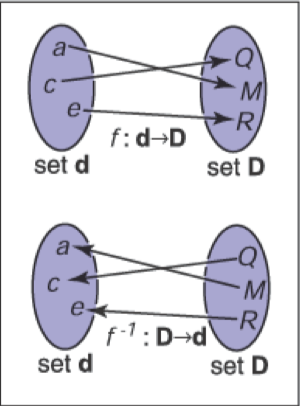
\includegraphics[width=0.58\textwidth]{2.1.png}
\caption{一个双射 $f$ 和反函数 $f^{-1}$。注意,$f^{-1}$也是一个双射。}
\end{minipage}
\begin{minipage}[t]{0.45\textwidth}
\centering
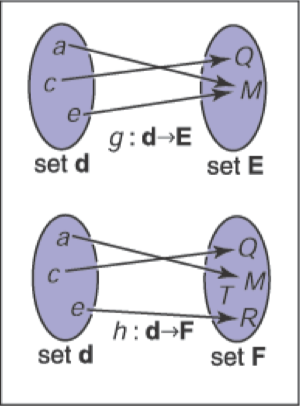
\includegraphics[width=0.58\textwidth]{2.2.png}
\caption{函数 $g$ 不具有反函数,因为\textbf{d}中的两个元素匹配到\textbf{E}中相同的元素。函数 $h$ 没有反函数因为\textbf{F}中的元素 $T$ 在\textbf{d} 中没有匹配的元素。}
\end{minipage}
\end{figure}

一个双射的例子是 $f : \mathbb{R} \mapsto \mathbb{R}$,其中 $f(x) = x^3$。它的反函数为 $f^{-1}(x) = \sqrt[3]{x}$ 。这个例子表明,标准的符号可能有些笨拙,因为 $x$ 在 $f$ 和 $f^{-1}$ 中都被用作虚拟变量。有时使用不同的虚拟变量会更直观,$y = f(x)$,$x=f^{-1}(y)$。这就产生了更直观的 $y = x^3$ 和 $x = \sqrt[3]{y}$。一个没有反函数的例子是 $sqr : \mathbb{R} \mapsto \mathbb{R}$,其中 $sqr(x) = x^2$。它不具有反函数的原因包括两个:首先 $x^2 = (-x)^2$,其次域中没有成员映射到目标的负数部分。请注意,如果我们把域和范围限制在 $\mathbb{R^+}$,可以定义一个反函数。那么 $\sqrt{x}$ 是一个有效的反函数。

\subsection{区间}

通常情况下,我们希望指定一个函数处理的是数值受限的实数。这样的一个约束就是指定一个区间。区间的一个例子是零和一之间的实数,不包括零或一。我们把它表示为 $(0,1)$。因为它不包括其端点,所以被称为开区间。相应的闭区间,包含其端点,用方括号表示: $[ 0 , 1 ]$ 。这种符号可以混合使用;即 $[0,1)$ 包括零,但不包括一。当写一个区间 $[a,b]$ 时,我们假定 $a \leq b$。表示一个区间的三种常见方法如图2.3所示。区间的笛卡尔积经常被使用。例如,为了表示点 $x$ 在三维的单位立方体中,我们说$x \in [0, 1]^3$。

\begin{figure}[htbp]
\centering
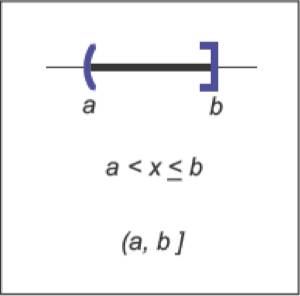
\includegraphics[width=0.26\textwidth]{2.3.png}
\caption{三个表示等效方式用于表示区间从 $a$ 到 $b$,包含 $b$ 但不包含 $a$}
\end{figure}

区间在与集合运算的结合中特别有用:交集、并集和差集。例如,两个区间的交集是它们共同点的集合。符号 $\cap$ 用来表示交集。例如,$[3,5) \cap [4,6] = [4,5)$。而并集,使用符号 $\cup$ 用来表示任何一个区间内的点。例如,$[3,5) \cup [4,6] = [3,6]$。与前两个运算符不同,差集运算符根据参数顺序产生不同结果。减号用于差集运算,它返回左侧区间中不在右侧区间的点。例如,$[3,5) - [4,6] = [3,4]$,以及 $[4,6] - [3,5] = [5,6]$。这些操作用区间图特别容易直观地表现出来(图2.4)。

\begin{figure}[htbp]
\centering
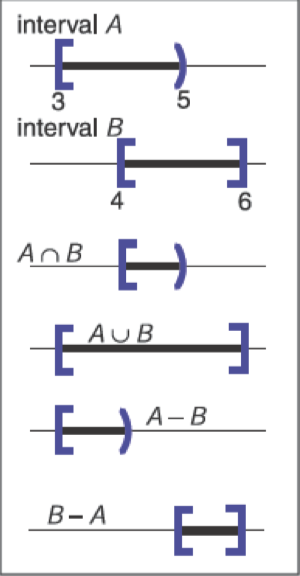
\includegraphics[width=0.26\textwidth]{2.4.png}
\caption{在 $[3,5)$ 和 $[4,6]$ 上的区间操作}
\end{figure}

\subsection{对数函数}

虽然当前不像计算器出现之前那样普遍,但对数通常在具有指数项的方程问题中很有用。根据定义,每个对数都有一个底 $a$。以 $a$ 为底的对数 $x$ 通常被写作 $\log_ax$,并且它被定义为若要得到 $x$ 需要将 $a$ 乘幂的指数值。即,

\begin{center}
$ y = \log_ax \iff a^y = x$。
\end{center}

请注意,以 $a$ 为底数的对数和将 $a$ 乘幂的函数是互逆的。这个基本定义导致几个后果:

\[
\begin{aligned}
a^{\log_a(x)} &= x; \\
\log_a(a^x) &= x; \\
\log_a(xy) &= \log_ax+\log_ay; \\
\log_a(x/y) &= \log_ax-\log_ay; \\
\log_ax &= \log_ab\log_bx.
\end{aligned}
\]

当我们将微积分应用于对数时,经常会出现特殊数字 $e=2.718...$。以 $e$ 为底的对数被称为自然对数。我们采用常用的简写 $ln$ 来表示:

\begin{center}
$\ln x \equiv \log_ex$。
\end{center}

请注意,“ $\equiv$ ”符号可以被理解为“根据定义恒等”。像 $\pi$ 一样,特殊数字 $e$ 出现在很多情况下。除了 $e$ 以外,在许多领域还使用特定的技术进行操作,并在其符号中省略基数,即 $\log x$。例如,天文学家经常使用以十为底,理论计算机科学家经常使用以二为底。由于计算机图形学借鉴了许多领域的技术,我们将避免这种缩写。

对数和指数的导数阐明了为什么自然对数是“自然的”:

\[
\begin{aligned}
\frac{d}{d x} \log _{a} x &=\frac{1}{x \ln a} \\
\frac{d}{d x} a^{x} &=a^{x} \ln a
\end{aligned}
\]

上面的常数乘数只有在 $a = e$ 时才是是统一的。

\section{求解二次方程}

一个二次方程满足如下格式

\begin{center}
$Ax^2+Bx+C=0$,
\end{center}

其中 $x$ 是一个未知的实数,并且 $A$、$B$ 和 $C$ 是已知的常数。如果你想到 $y=Ax^2+Bx+y$ 的二维 $xy$ 图,那么解就是任何 $x$ 值在 $y$ 中的“零交叉”。因为 $y=Ax^2+Bx+y$ 是一条抛物线,根据抛物线是否未相交、相切或相交于 $x$ 轴,将有零个、一个或两个实数解(图2.5)。

\begin{figure}[htbp]
\centering
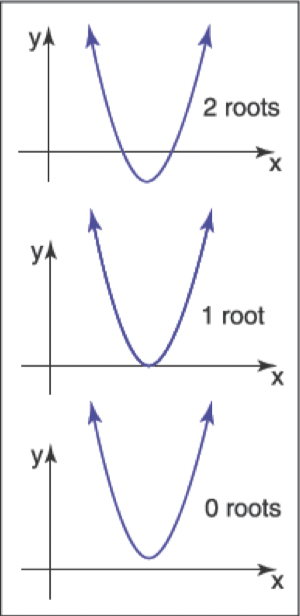
\includegraphics[width=0.26\textwidth]{2.5.png}
\caption{二次方程根的几何解释是抛物线与 $x$ 轴的交点。}
\end{figure}

\section{三角学}

\section{矢量图}

\section{积分}

\section{密度函数}

\section{曲线和曲面}

\section{线性插值}

\section{三角形}

\section{离散概率}

\section{连续概率}

\section{蒙特卡洛积分}

\chapter{光栅图像}

\section{光栅设备}

\section{图像、像素和几何}

\section{RGB颜色}

\section{阿尔法合成}

\chapter{光线追踪}

\section{基础光线追踪算法}

\section{透视图}

\section{计算视线}

\section{光线相交}

\section{阴影}

\section{历史笔记}

\chapter{表面着色}

\section{点状光源}


\section{基本反射模型}


\section{环境照明}


\end{document}
